\documentclass[a4paper, 7pt]{article}
\usepackage{geometry}
%% % Geometry: es para modificar los márgenes del documento
\usepackage[left=3cm, right=2.5cm, top=2.5cm, bottom=2.5cm]{geometry}
%% lipsum: para generar texto de ejemplo. Se puede eliminar una vez que se eliminen todos los \lipsum[] del documento.
\usepackage{lipsum}
% lscape: en caso de querer rotar una hoja, buscar información en internet en caso de ser requerido. 
\usepackage{lscape}
\usepackage{float}
% inputenc: para que latex acepte caracteres latinos como los acentos y la letra ñ.
\usepackage[utf8]{inputenc}
% babel: para traducir los títulos que vienen originalmente en inglés. Ejemplo: Fecha, Chapter, Bibliography, Appendix, etc.
\usepackage[spanish,es-tabla]{babel}
% natbib: para poder citar utilizando paréntesis redondos con \citep{•} o sin parentesis con \cite{•}
\usepackage[numbers]{natbib}
\usepackage{float} % para usar [H] y obligar que las figuras o tablas aparezcan donde es requerido.
\usepackage[pdftex]{graphicx} % graphicx: para incorporar imágenes. Recordar que las imágenes 'gif' no son aceptadas por Latex, se sugiere utilizar formato png por su calidad, en segunda intantcia jpg.
\usepackage{parskip} % parskip: par no dejar sangrías e insertar espacios entre párrafos en su lugar.
\usepackage{amsmath} %paquete para escribir fórmulas matemáticas.
\usepackage{amsfonts}%paquete para escribir fórmulas matemáticas.
\usepackage{amssymb} %paquete para escribir fórmulas matemáticas.
\usepackage{amsbsy}
\usepackage{upgreek}
\usepackage[usenames,dvipsnames,svgnames,table]{xcolor} %xcolor: para definir colores y dar color a tablas.
\usepackage{multirow}

\graphicspath{ {figures/} }
\usepackage{array}

% hyperref: define opciones especiales para el documento PDF producido.
\usepackage[pdftex, bookmarksnumbered,  pagebackref, colorlinks=true, citecolor=DarkBlue, linkcolor=DarkBlue!30!Black, urlcolor=Black,bookmarksopen]{hyperref}

% El paquete fancyhdr es para definir opciones de encabezado y pié de página
% Según el formato existente a la fecha (agosto de 2015) esto no se considera
% Su utilización en este caso es para situar el número de página en la parte
% inferior derecha de la página.

\usepackage{fancyhdr} % activamos el paquete
	\pagestyle{fancy} % seleccionamos un estilo
	\lhead{} % texto izquierda de la cabecera
	\chead{} % texto centro de la cabecera
	\rhead{\textcolor[gray]{0.5}{\textit{\nouppercase \leftmark}}} % Nombre del capítulo. \nouppercase: uso de minúsculas
	\lfoot{} % texto izquierda del pie
	\cfoot{} % imagen centro del pie
	\rfoot{\textcolor[gray]{0.5}{\thepage}} % Número de página a la derecha, abajo
	\renewcommand{\headrulewidth}{0.2pt} % grosor de la línea de la cabecera

\fancypagestyle{detailed}{
    \fancyhf{} % clear all header and footers
    \fancyfoot[R]{\textcolor[gray]{0.5}{\thepage}}
	%\fancyhead{}    
    \renewcommand{\headrulewidth}{0pt}
 }
 
\usepackage{etoolbox}
\patchcmd{\chapter}{\thispagestyle{plain}}{\thispagestyle{detailed}}{}{}

%times: para uar letra tipo Times New Roman
\usepackage{times}

%separación entre líneas (1.2 espacios). En word es interlineado exacto a 12 pts
\renewcommand{\baselinestretch}{1.2} 

\usepackage{titlesec} % para poder modificar los títulos

% Para la numeración de tablas y figuras.
\renewcommand\thefigure{\arabic{section}.\arabic{figure}} % Genera numeración X.Y
\renewcommand\thetable{\arabic{section}.\arabic{table}} % Genera numeración X.Y
\numberwithin{figure}{section} %Hace que la primera figura de cada sección X sea X.1
\numberwithin{table}{section} %Hace que la primera tabla de cada sección X sea X

\usepackage{booktabs} % Para trabajar con opciones especiales de tablas.
\usepackage{caption}

\usepackage{setspace}

% El índice de tablas e imágenes se superpone el texto al número de la figura o tabla.
% Esta configuración arregla dicho problema, modificar el 3.0 de ser necesario.
\usepackage{tocloft}
\addtolength{\cftfignumwidth}{3.0em}
\renewcommand{\cftfigpresnum}{\figurename\ }
\addtolength{\cfttabnumwidth}{3.0em}
\renewcommand{\cfttabpresnum}{\tablename\ }
\usepackage[utf8]{inputenc}
\usepackage{amssymb}
\usepackage{graphicx, wrapfig, subcaption, setspace, booktabs}
\usepackage{lscape}
\usepackage{float}
\usepackage{changepage}
\usepackage{capt-of}
\usepackage{wrapfig}
\usepackage{listings}
\usepackage{amsmath}

\begin{document}

\begin{titlepage}
		\begin{center}
		\vspace{5 mm}\textbf{\Large UNIVERSIDAD POLITÉCNICA DE MADRID} \par
		\vspace{10 mm}
      			\begin{figure}[htb]
				\begin{center}
					
\includegraphics[scale=0.3]{./images/logo-upm.eps}
				\end{center}
			\end{figure}\par
  
      %\vspace{10 mm}\textbf{\large \degree} \par
      %\vspace{10 mm}\textbf{\large \faculty} \par
      %\vspace{20 mm}\textbf{\large \department } \par


      \vspace{20 mm}\textsc{\Large Homework 2 \\ Modelo de regresión para los precios de diamantes } \par
      
      \vspace{10 mm}\textsc{STATISTICAL DATA ANALYSIS}\par
      \vspace{10 mm}\textsc{AUTORES: \\ Cristian Abrante Dorta, \\ Álvaro Arranz Domínguez, \\ Ángel González López, \\ Daniel Saiz González}\par
		
	\rule{80mm}{0.1mm}\\      
      
	  \vspace{10 mm}
      \textsc{Master's Programme in ICT Innovation: Data Science}\par 
      %\vfill\textrm{\address. \hfill \monthyear}
      
      
      \vspace{10 mm}\textsc{ESCUELA TÉCNICA SUPERIOR DE INGENIERÍA DE INFORMÁTICA}		
		\end{center}
\end{titlepage}


\newgeometry{textwidth=18cm,textheight=27cm}

\section{Descripción del conjunto de datos}
\label{sec:descripcion-datos}
\noindent

El conjunto de datos que estudiaremos se trata de una lista de 308 piedras preciosas. Este conjunto de datos se ha creado con fines educativos e incluye las siguientes variables:

\begin{itemize}
    \item \texttt{caratage}: Esta variable numérica continua se refiere a los quilates que posee el diamante, unidad de medida utilizada para pesar gemas y otras piedras preciosas. La correspondencia es de 1 quilate con 0.2 gramos.
    \item \texttt{purity}: Nivel de pureza del color del diamante. Varía desde el nivel \textbf{D} hasta el \textbf{I}, donde el \textbf{D} se corresponde con el nivel más puro.
    \item \texttt{clarity}: Nivel de claridad del diamante. Se corresponde con los valores: \textbf{IF, VVS1, VVS2, VS1, VS2}, ordenados de mejor a peor.
    \item \texttt{certificate}: Certificado de calidad emitido por una institución de renombre. Puede tener los siguientes valores: \textbf{GIA, IGI y HRD}.
    \item \texttt{price}: Precio que tiene el diamante, expresado en dólares de Singapur.
\end{itemize}

\section{Preguntas de investigación}
\noindent
El objetivo de esta investigación es dar respuesta al conjunto de preguntas formuladas aplicando diferentes técnicas de visualización y transformación de datos.

%%%%%%%%%%%%%%%%%%%%%%%%%%%%%%%%%%%%%%%%%
%   Pregunta 1
%%%%%%%%%%%%%%%%%%%%%%%%%%%%%%%%%%%%%%%%%
\subsection{Representa la gráfica \texttt{price} vs. \texttt{caratage} y la gráfica \texttt{log(price)} vs \texttt{caratage}. Decide que variable de respuesta es mejor utilizar.}
\label{subsec:question-1}

En primer lugar, representaremos ambas gráficas:

\begin{figure}[h!]
  \centering
  \begin{subfigure}[b]{0.25\linewidth}
    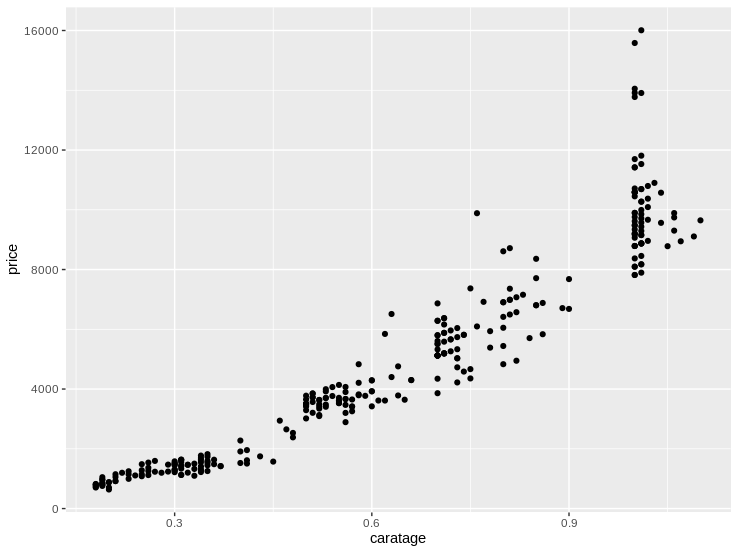
\includegraphics[width=\linewidth]{report/images/question-1/price.png}
    \caption{\texttt{price} vs \texttt{caratage}}
  \end{subfigure}
  \begin{subfigure}[b]{0.25\linewidth}
    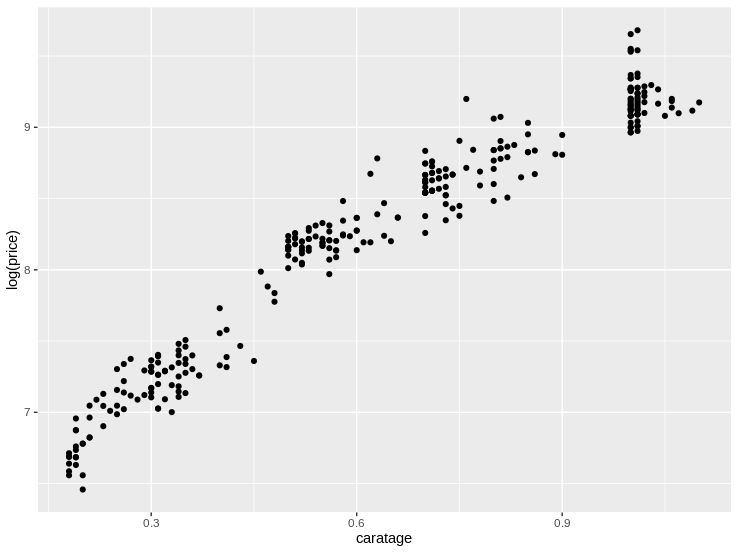
\includegraphics[width=\linewidth]{report/images/question-1/logprice.png}
    \caption{\texttt{log(price)} vs \texttt{caratage}}
  \end{subfigure}
  \caption{Gráficas para \texttt{price} y \texttt{caratage}}
  \label{fig:coffee}
\end{figure}

A simple vista, se puede apreciar que existe una relación lineal mucho mayor entre las variables \texttt{log(caratage)} y \texttt{price}, que entre \texttt{caratage} y \texttt{price}. Sin embargo, esto no es motivo suficiente para decantarnos por una variable u otra. Para determinar cual elegiremos finalmente se representará el histograma de ambas.

\begin{figure}[h!]
  \centering
  \begin{subfigure}[b]{0.25\linewidth}
    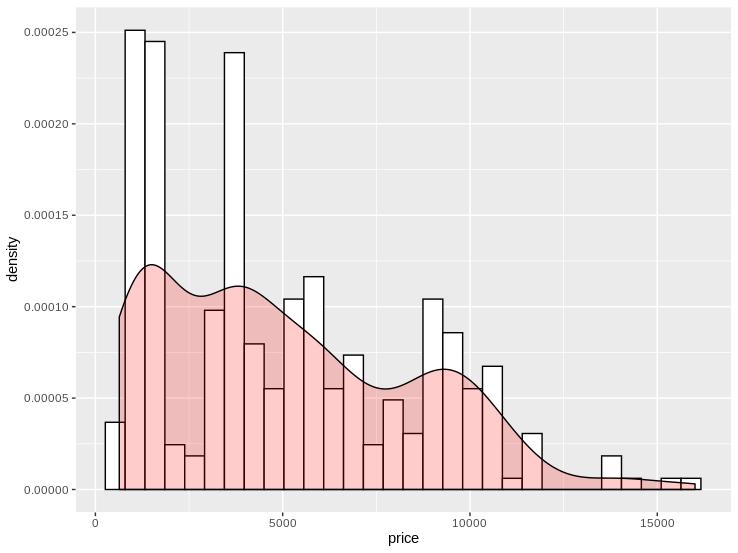
\includegraphics[width=\linewidth]{report/images/question-1/histogram-price.png}
    \caption{Histograma y representación de la densidad para la variable \texttt{price}}
  \end{subfigure}
  \begin{subfigure}[b]{0.25\linewidth}
    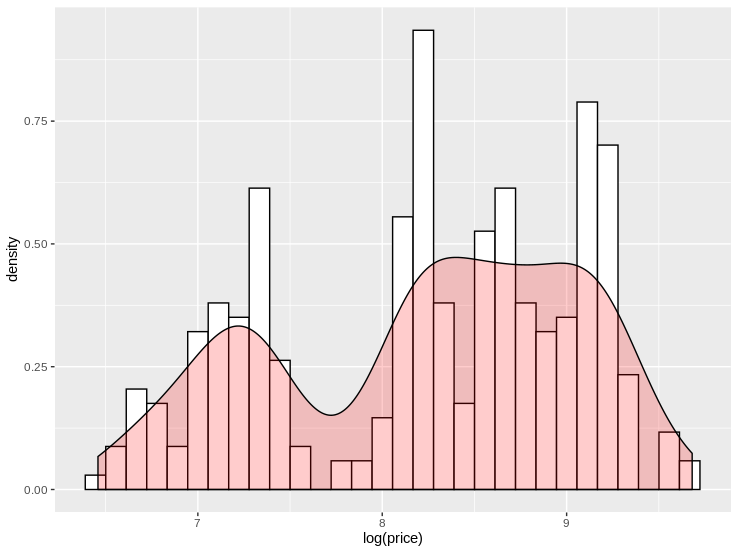
\includegraphics[width=\linewidth]{report/images/question-1/histogram-logprice.png}
    \caption{Histograma y representación de la densidad para la variable \texttt{log(price)}}
  \end{subfigure}
  \caption{Histogramas para \texttt{price} y \texttt{caratage}}
  \label{fig:coffee}
\end{figure}

En el histograma de la variable \texttt{price} se puede ver claramente una desviación (\textit{skewed}) hacia el lado izquierdo. Sin embargo, en la representación logarítmica de la variable, se puede observar que la distribución se aproxima más a una distribución normal. Aunque la normalidad de la variable independiente no es una suposición indispensable para llevar a cabo un modelo de regresión lineal, es preferible que nuestra variable de respuesta cumpla esta condición. Es por ello que para nuestro estudio utilizaremos la variable \textbf{log(price)}. \\

Cabe destacar una desventaja de la elección de esta variable dependiente, y es la \textbf{interpretabilidad}. De manera general, el modelo que vamos a ajustar tendrá la siguiente forma:

\begin{equation}
    log(Y) = \alpha + \widehat{\beta}X + \epsilon
\end{equation}

Como todos los modelos lineales, un incremento de una unidad en la variable $x_i$ supondría un incremento de la variable de respuesta $log(Y)$ en $\beta_i$ unidades. Pero esto no resulta demasiado clarificador respecto a la variable $Y$, por tanto, deberemos utilizar las propiedades de los logaritmos para establecer estas dos interpretaciones:

\begin{itemize}
    \item Un incremento de una unidad en la variable $x_i$, se traduce en la multiplicación de la variable de respuesta $Y$ por $e^{\beta_i}$.
    \item Para valores pequeños de $\beta_i$, se puede considerar que $e^{\beta_i} \approx 1 + \beta_i$ y de esta forma, interpretar la multiplicación como un incremento porcentual. Por ejemplo para $\beta_i = 0.05$, podemos decir que $e^{0.5} \approx 1.05$ y por tanto el incremento en la variable $Y$ será de un $5\%$ aproximadamente.
\end{itemize}

%%%%%%%%%%%%%%%%%%%%%%%%%%%%%%%%%%%%%%%%%
%   Pregunta 2
%%%%%%%%%%%%%%%%%%%%%%%%%%%%%%%%%%%%%%%%%
\subsection{Encuentra una manera adecuada de incluir, además de \texttt{caratage}, la otra información categórica disponible: \texttt{clarity}, \texttt{purity} y \texttt{certificate}. Comenta el modelo que se ha ajustado, realizando un análisis básico de los residuos.}
\label{subsec:question-2}

Para poder incluir la información de las variables categóricas disponibles se ha tenido que comprobar, en primer lugar, qué categoría aparecía de referencia en cada una de ellas. En este caso se han usado el peor nivel de \textit{purity} y de \textit{clarity}, que son “I” y “VS2”, respectivamente. En el caso del \textit{certificate} se ha establecido “HRD” como referencia.
Una vez establecidas las categorías de referencia, se ha formado el modelo lineal con \textit{caratage} como variable numérica y el resto como variables categóricas, en el que se ha obtenido un estimador beta por cada categoría.

\begin{figure}[h!]
    \centering
    \begin{tabular}{c}
        \begin{lstlisting}[basicstyle=\tiny, language=r]
               Coefficients:
                Estimate Std. Error t value Pr(>|t|)    
(Intercept)     6.077239   0.048091 126.369  < 2e-16 ***
caratage        2.855013   0.036968  77.230  < 2e-16 ***
purityD         0.416557   0.041382  10.066  < 2e-16 ***
purityE         0.387047   0.030824  12.557  < 2e-16 ***
purityF         0.310198   0.027479  11.288  < 2e-16 ***
purityG         0.210207   0.028359   7.412 1.32e-12 ***
purityH         0.128681   0.028523   4.511 9.31e-06 ***
clarityIF       0.298541   0.033303   8.964  < 2e-16 ***
clarityVS1      0.096609   0.024919   3.877  0.00013 ***
clarityVVS1     0.297835   0.028102  10.598  < 2e-16 ***
clarityVVS2     0.201923   0.025344   7.967 3.56e-14 ***
certificateGIA  0.008856   0.020864   0.424  0.67155    
certificateIGI -0.173855   0.028673  -6.063 4.07e-09 *** 
        \end{lstlisting}
    \end{tabular}
    \caption{Tabla que muestra el output para el modelo lineal que se ha ajustado}
    \label{fig:summary_model}
\end{figure}

A la vista de los resultados de este primer modelo generado, se ha observado que el $p-valor$ de la variable "GIA" de  \textit{certificate} es de 0.67, con lo cual esta no es significativa. Como podemos ver, el precio se ve sustancialmente incrementado por un incremento unitario en el valor de los quilates. Seguidamente, cada uno de los valores de pureza se corresponde con un incremento porcentual que varía desde un 41\% de incremento del valor para el valor de pureza D hasta un 13\% para el valor H. Ocurre algo similar pero para el valor de claridad del color. En el caso en el que se tenga una certificación "IGI", el precio se reduce debido a que el signo del estimador es negativo. Esto puede ser indicativo de la menor reputación de esta institución respecto a la de referencia. Seguidamente se han realizado análisis para estudiar la normalidad, la varianza y la independencia de los residuos. Se han observado las gráficas de diagnóstico  y se han realizado tests para cada una de las propiedades que se quieren estudiar.

\begin{figure}[H]
  \centering
  \begin{subfigure}[b]{0.5\linewidth}
    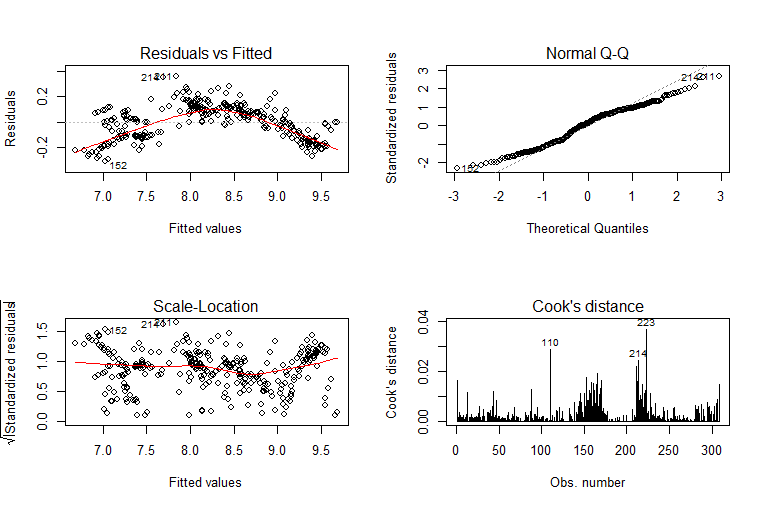
\includegraphics[width=\linewidth]{report/images/question-2/Rplot.png}
    \caption{Figura 4: Gráficas de diagnóstico del modelo lineal}
  \end{subfigure}
  \label{fig:coffee}
\end{figure}

En primer lugar estudiaremos la \textbf{normalidad} de los residuos. Para ello, se ha utilizado la prueba de \textit{Jarque Bera} \cite{jarquebera}.\\

Obteniendo un un $p-valor$ de 0.01775. Esto nos permite rechazar la hipótesis nula, es decir que los residuos no son normales y existe un cierto patrón en ellos. Esto también se puede observar en la primera gráfica, en la que se puede ver que los residuos no siguen una distribución aleatoria y por tanto la linea roja no es horizontal y centrada en el 0. Para la \textbf{independencia de los residuos}, se ha utilizado el test de \textit{Durbin-Watson}, obteniendo un valor de 0.31 y un $p-valor$ de 2.2e-16, lo cual indica que no existe independencia entre los residuos. Finalmente utilizaremos el test de \textit{Breusch-Pagan} para comprobar la \textbf{igualdad de varianzas}, obteniendo un $p-valor$ de 4.265e-06. Esto nos indica que existen problemas de homoceidasticidad entre los residuos. \\

Además, comprobaremos la existencia de outliers mediante la función \texttt{outlierTest}, la cual nos da como resultado que la observación 211 es un outlier. Al existir tampocos outliers, no podemos concluir que los errores en la normalidad se deban a ellos. Como podemos comprobar, ninguna de las suposiciones se cumplen con este modelo.

%%%%%%%%%%%%%%%%%%%%%%%%%%%%%%%%%%%%%%%%%
%   Pregunta 3
%%%%%%%%%%%%%%%%%%%%%%%%%%%%%%%%%%%%%%%%%
\subsection{Crea dos acciones para remediar el resultado anterior}
\label{subsec:question-3}

\subsubsection{Crear una nueva variable categórica para segregar las piedras según caratage. Añadir esta nueva variable al modelo existente, así como un término de interacción entre esta nueva variable y caratage.}

Para arreglar la situación anterior, hemos creado una variable categórica respecto al valor de \texttt{caratage}. Para crear esta variable (\texttt{caratageCategorical}), se ha seguido el siguiuente criterio:

\begin{itemize}
    \item Si el valor de la variable es inferior a 0.5 se considera una piedra pequeña y se asigna el valor \texttt{small}.
    \item Si el \texttt{caratage} está entre 0.5 y 1.0 se considera un valor mediano y se asigna el valor \texttt{medium}.
    \item Si el \texttt{caratage} es mayor que 1.0 se asigna el valor \texttt{large}.
\end{itemize}

Estableciendo este criterio, y añadiendo una variable de interacción entre el \texttt{caratage} numérico y el categórico, se ha ajustado este modelo, que podemos observar mediante la función \texttt{summary}.

\begin{figure}[H]
    \centering
    \begin{tabular}{c}
        \begin{lstlisting}[basicstyle=\tiny, language=r]
                                    Estimate Std. Error t value Pr(>|t|)    
(Intercept)                         5.530676   0.032878 168.218  < 2e-16 ***
caratage                            4.257150   0.085503  49.790  < 2e-16 ***
purityD                             0.433562   0.016897  25.659  < 2e-16 ***
purityE                             0.348679   0.012550  27.784  < 2e-16 ***
purityF                             0.272843   0.011142  24.488  < 2e-16 ***
purityG                             0.187887   0.011522  16.307  < 2e-16 ***
purityH                             0.107866   0.011481   9.395  < 2e-16 ***
clarityIF                           0.311385   0.013543  22.992  < 2e-16 ***
clarityVS1                          0.068240   0.010060   6.783 6.56e-11 ***
clarityVVS1                         0.213344   0.011536  18.493  < 2e-16 ***
clarityVVS2                         0.134180   0.010351  12.963  < 2e-16 ***
certificateGIA                      0.007703   0.008473   0.909    0.364    
certificateIGI                     -0.016726   0.012177  -1.374    0.171    
caratageCategoricalmedium           0.946026   0.039091  24.201  < 2e-16 ***
caratageCategoricallarge            2.376272   0.319800   7.430 1.21e-12 ***
caratage:caratageCategoricalmedium -1.765492   0.093498 -18.883  < 2e-16 ***
caratage:caratageCategoricallarge  -3.259971   0.323445 -10.079  < 2e-16 ***
        \end{lstlisting}
    \end{tabular}
    \caption{Tabla que muestra el output para el modelo lineal con \texttt{caratageCategorical}}
    \label{fig:summary_model}
\end{figure}

Como podemos observar, en este modelo la variable categoríca \texttt{certificate} no tiene relevancia cuando la institución que concede el certificado es GIA e IGI, debido a los altos valores del $p-valor$.


\subsubsection{¿Es satisfactorio este modelo de regresión? ¿Se validan los supuestos estándar de la regresión lineal? ¿Son razonables las estimaciones numéricas?}

Para garantizar si es satisfactorio este modelo lineal, representaremos las gráficas de los residuos, y sobre ellas comprobaremos los supuestos del modelo de regresión. En primer supuesto es la \textbf{relación lineal} entre las variables independientes y la variable respuesta. Para ello, nos fijaremos en la primera gráfica, que representa los residuos respecto a los valores predichos. Para que se cumpla la relación lineal, los residuos tienen que ser aleatorios y seguir una distribución normal, y por tanto la línea roja debe ser aproximadamente horizontal y centrada en el valor 0. Lo cual se cumple en comparación con el modelo del ejercicio anterior. El segundo supuesto es la \textbf{independencia de los residuos}. Utilizamos el test de \textit{Durbin Watson}, para comprobar los valores. El resultado del test es de 1.03, con un $p-valor$ de 2.2e-16, lo cual nos indica que existe correlación entre los residuos y que por tanto no son independientes. Sin embargo, este valor es superior al 0.31 obtenido en el ejercicio anterior. Seguidamente, comprobaremos la \textbf{normalidad de los residuos}. Esto se puede comprobar visualmente en la gráfica Normal QQ-Plot, pues los residuos siguen la recta y por tanto son normales. Para una comprobación numérica se utiliza el test \textit{jarque-Bera} \cite{jarquebera}, el cual nos da un $p-valor$ de 0.5111, lo que implica que existe normalidad en los residuos, pudiendo rechazar la hipótesis nula. \\

Finalmente, comprobaremos la igualdad de las varianzas. En la imagen se corresponde con el tercer gráfico, el cual debería seguir de manera aproximada una linea recta horizontal, lo cual no se cumple. De manera numérica utilizamos el test de \textit{Breuch-Pagan}, el cual nos da un $p-valor$ de 4.117e-07, con lo cual podemos afirmar que existe un grado de homoceidasticidad en nuestros residuos.

\begin{figure}[h!]
    \centering
    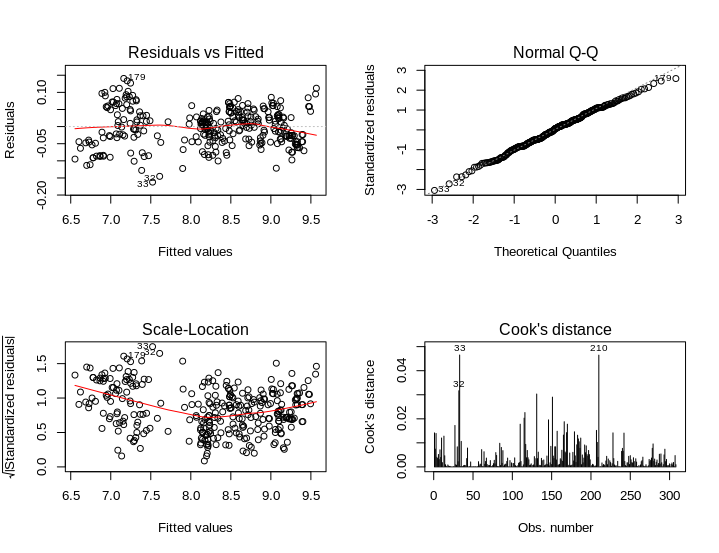
\includegraphics[scale=0.5]{report/images/question-3/question-1.png}
    \caption{Residuals on model with categorical \texttt{caratage}}
    \label{fig:my_label}
\end{figure}

\subsubsection{Interpretar el parámetro de interacción. ¿Qué podemos inferir sobre el precio incremental del caratage en los 3 grupos?}

En primer lugar, podemos comprobar que el parámetro de interacción es significativo, puesto que el $p-valor$ de ambos términos es menor a 0.05.  Para diamantes con valor \texttt{small}, al ser la variable de referencia todo el incremento se reune en el término \texttt{intercept}, además del propio valor añadido por \texttt{caratage}. Para el grupo \texttt{medium}, al incremento dado por \texttt{caratage}, tenemos que restarle -1.76. Aunque también tenemos que tener en cuenta lo que aporta la variable categórica al resultado. Finalmente, para el grupo \texttt{large}, se debe restar -3.25 al valor aportado por \texttt{caratage}. Aunque esto pueda parecer contradictorio, tiene sentido puesto que la existencia de la variable categórica está aportando a su vez un valor de 2.37 a la variable de respuesta.

\subsubsection{¿Qué es más valorado: el color(\texttt{purity}) o la claridad \texttt{clarity}? }

En términos absolutos, cuando se tiene la mejor categoría de pureza de color (D), se tiene un valor de 0.43, lo cual significa que se aumenta el precio del diamante en un 43\%. Por el contrario, en cuanto a la claridad (\texttt{clarity}), el mejor valor que se puede obtener (IF), aumenta el precio del diamante en un 31\%.  Con lo cual se puede determinar que el color es mucho mas valorado que la claridad.

\subsubsection{Siendo todas las demás variables iguales, ¿cuál es la diferencia de precio medio entre un diamante de grado D y otro de grado (a) I (b) E? }

Cuando se tiene un grado de pureza D un diamante aumenta su valor en un 43\%. A diferencia de uno de tipo I, el cual al ser la variable de referencia, tiene solo su valor incluido en el término \texttt{Intercept}, con lo cual concluimos que el valor es un 43\% mayor. En comparación con un diamante de grado E, el cual aporta un 34\% al precio, podemos afirmar que uno de grado D tiene un valor un 9\% superior.

\subsubsection{Siendo todas las demás variables iguales, ¿existen diferencias de precio entre las piedras evaluadas por el GIA, el IGI y el HRD? }

Teniendo en cuenta el modelo que hemos ajustado, en el se puede comprobar que el certificado con valor GIA e IGI no es significativo, con lo cual realmente no existe una diferencia sustancial de precio, e incluso se debería eliminar del modelo. 

\subsubsection{Añade el cuadrado de \texttt{caratage} como una nueva variable explicatoria.}

Si añadimos el cuadrado de \texttt{caratage} como variable independiente, y realizamos el \texttt{summary} obtenemos el resultado de la tabla \ref{fig:summary_model1}. Tal y como ocurría en el caso anterior, los valores de certificado pueden ser eliminados debido a que su $p-valor$ no es significante. Para comprobar si cumple las suposiciones del modelo, realizaremos las gráficas \ref{fig:my_label1}. Primero comprobaremos que existe una \textbf{relación lineal} entre los datos, para ello, observamos la primera gráfica, y teniendo en cuenta el caso anterior, si la linea roja es horizontal y se extiende a lo largo del valor 0 es indicativo de que existe una relación lineal entre las variables. En segundo lugar, comprobaremos la \textbf{independencia} de los residuos. Para ello utilizamos el test de \textit{Durbin Watson}, obteniendo un valor de 0.98 y un $p-valor$ de 2.2e-16. Con lo cual no podemos garantizar que existe independencia entre los residuos, y obteniendo un valor ligeramente peor que en el anterior modelo, pero mucho mejor que el modelo original que queremos arreglar.\\

\begin{figure}[h!]
    \centering
    \begin{tabular}{c}
        \begin{lstlisting}[basicstyle=\tiny, language=r]
                Estimate Std. Error t value Pr(>|t|)    
(Intercept)     5.306339   0.029611 179.200  < 2e-16 ***
caratage        5.670616   0.079284  71.523  < 2e-16 ***
purityD         0.442606   0.017742  24.947  < 2e-16 ***
purityE         0.363359   0.013220  27.485  < 2e-16 ***
purityF         0.286615   0.011789  24.311  < 2e-16 ***
purityG         0.197573   0.012153  16.257  < 2e-16 ***
purityH         0.103508   0.012238   8.458 1.30e-15 ***
clarityIF       0.320183   0.014279  22.424  < 2e-16 ***
clarityVS1      0.075713   0.010690   7.083 1.05e-11 ***
clarityVVS1     0.226174   0.012199  18.540  < 2e-16 ***
clarityVVS2     0.143481   0.010976  13.072  < 2e-16 ***
certificateGIA  0.006223   0.008938   0.696    0.487    
certificateIGI -0.019190   0.013003  -1.476    0.141    
I(caratage^2)  -2.102922   0.058022 -36.243  < 2e-16 ***
        \end{lstlisting}
    \end{tabular}
    \caption{Tabla que muestra el output para el modelo lineal con \texttt{caratageCategorical}}
    \label{fig:summary_model1}
\end{figure}

\begin{figure}[h!]
    \centering
    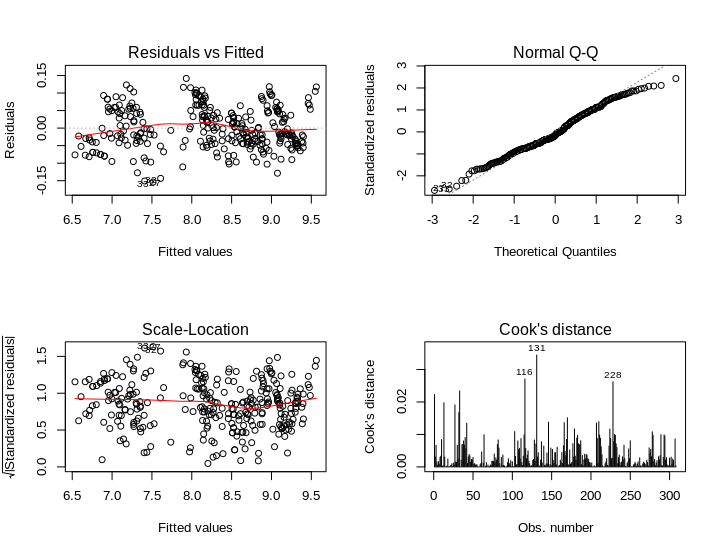
\includegraphics[scale=0.5]{report/images/question-3/residuals-squared.png}
    \caption{Residuals on model with categorical \texttt{caratage}}
    \label{fig:my_label1}
\end{figure}

Luego, comprobaremos la \textbf{normalidad de los residuos}. Al igual que en el caso anterior, esto se comprueba en la gráfica QQ plot, en la que vemos que los residuos siguen la linea. También se utilizará el test de \textit{Jarque Bera} \cite{jarquebera}, para una comprobación numérica. Hemos obtenido un $p-valor$ de 0.14, con lo cual podemos rechazar la hipótesis de que los residuos no son normales. Finalmente, comprobaremos la \textbf{igualdad de varianzas}. Esto se puede ver en la tercera gráfica, mediante la línea roja. A su vez se ha utilizado el test de \textit{Breusch-Pagan}. En el hemos obtenido un $p-valor$ de 0.2441 lo cual nos permite rechazar la hipótesis de que existe homoceidasticidad en los residuos.

%%%%%%%%%%%%%%%%%%%%%%%%%%%%%%%%%%%%%%%%%
%   Pregunta 4
%%%%%%%%%%%%%%%%%%%%%%%%%%%%%%%%%%%%%%%%%
\subsection{¿Cuál de las acciones anteriores prefieres y por qué? Justifica la respuesta en términos de interpretabilidad y validez de los supuestos.}
\label{subsec:question-4}

En términos de validez de supuestos, hemos comprobado que la segunda aproximación es mucho más efectiva. En cuanto a la independencia de los residuos, hemos comprobado que ninguno de los modelos cumple esta condición, siendo el segundo modelo en cierta medida peor (con un resultado de 0.98 en el test de \textit{Durbin Watson}). En términos de normalidad de los residuos, hemos comprobado que ambos cumplen en esta condición. Finalmente, ha sido la suposición de igualdad de varianzas la que ha hecho que nos hayamos decantado por el segundo modelo, pues se ha demostrado que existe cierto grado de homoceidasticidad en los residuos del primer modelo (mediante el test de \textit{Breusch-Pagan}). En términos de interpretabilidad, tiene sentido que el precio de un diamante se incremente exponencialmente con el valor de caratage (modelo 2), pero tiene menos sentido que, partiendo del modelo que ya teníamos, que incluía la variable caratage, añadiendo una variable categorica que represente umbrales de tamaño de esta variable (modelo 1) tenga algún impacto positivo en el modelo.\\

Por ambos motivos, hemos decidido que la segunda aproximación es más acertada.

%%%%%%%%%%%%%%%%%%%%%%%%%%%%%%%%%%%%%%%%%
\begin{thebibliography}{9}
\bibitem{jarquebera}
    Jarque, Carlos M., and Anil K. Bera
    \newblock {\em Efficient tests for normality, homoscedasticity and serial independence of regression residuals}, 1980.
    
\bibitem{durbinwatson}
    Durbin, James, and Geoffrey S. Watson
    \newblock {\em Testing for serial correlation in least squares regression. II.}, 1951.

\end{thebibliography}

\end{document}